\documentclass[a4paper]{article}
\usepackage[latin1]{inputenc}
\usepackage[]{graphicx}
\usepackage{float}
\usepackage[]{comment}
\usepackage[]{parskip}
\usepackage{amsmath}
\usepackage{tabulary}
\usepackage{hyperref}

\title{MNXB01 HW2a}
\author{Emelie Olsson}

\usepackage{titlesec}

%F�r att ha mindre storlek p� section-text


\begin{document}

\maketitle

\begin{center}
\texttt{em6708ol-s@student.lu.se}
\end{center}

\section{Introduction}

This is introduction. The summary will be given in Section \ref{sec:about}.


\section{About Linux}\label{sec:about}
\begin{figure}[H]
\begin{center}
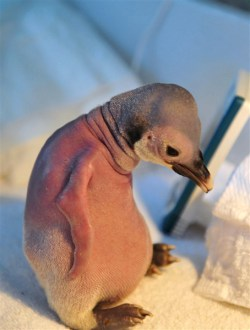
\includegraphics{ful-pingvin.jpg}
\end{center}
\caption{Penguin symbolizes Lunix}
\label{fig:penguin}
\end{figure}

Figure \ref{fig:penguin} shows a \textit{penguin}. For more details, check the Linux Web Page \cite{linuxwebb}.

\subsection{Linux flavours}
\label{sec:flavours}

Table \ref{tab:flavours} lists some Linux flavours \footnote{Only one is shown for simplicity}.

\begin{table}[H]
\begin{center}
\label{tab:flavours}
\begin{tabular}{|c|c|c|c|}
\textbf{Distribution}&RedHat&Debian&SuSE\\ \hline \hline
Fedora 20 & X & & \\ \hline
\end{tabular}
\caption{Different flavours of Linux}
\end{center}
\end{table}

\section{About mathematics}

Subscripts and superscripts: $A_x$, $A_{xy}$, $e^x$ and $e^{x^2}$. Using \_ outside math without \textbackslash \: causes big\_troubles.

Special symbols: $\alpha$, $\beta$, $\gamma$, $\delta$, $\sin x$, $\hbar$, $\lambda$, $\ldots$
More information can be found in Ref. \cite{latex}.

Equation \ref{eq:chi2} shows $\chi^2$.

\begin{equation}
\label{eq:chi2}
\chi^2 = \sum \limits_i \left (\frac{F_i-D_i}{\sigma_i} \right )^2
\end{equation}

\section{Summary}
\label{sec:summary}

We learned the following:
\begin{itemize}
\item Linux is good
\item \LaTeX \ is good for:
\begin{enumerate}
\item Structuring documents
\item Writing mathematical equations
\end{enumerate}
\end{itemize}

We can also write unformatted text:

\begin{verbatim}
\usepackage{verbatim}
Very useful if you want to include code, for example from Matlab. 
\end{verbatim}



\begin{thebibliography}{99}
\bibitem{linuxwebb} Linux web site: \url{www.linux.com}
\bibitem{latex} Leslie Lamport, \textsl{LaTeX: A Document Preparation System}, second edition, Addison-Wesley (1994).
\end{thebibliography}

\end{document}